\documentclass[12pt]{article}
%Gummi|065|=)
\usepackage{amsmath, amsfonts, amssymb}
\usepackage[landscape, margin=0.5in]{geometry}
\usepackage{xcolor}
\usepackage{graphicx}
\newcommand{\off}[1]{}
\DeclareMathSizes{20}{30}{21}{18}

\usepackage{tikz}

\title{\textbf{ Unipotent Flows }}
\author{John D Mangual}
\date{}
\begin{document}

\fontfamily{qag}\selectfont \fontsize{25}{30}\selectfont

\maketitle

% note AVOID THE WORDS 'Ratner Theorem' instead explain what it is

\noindent 

\newpage

\noindent \textbf{The matrix $\left(\begin{array}{cc}
1 & 1 \\ 0 & 1 \end{array} \right) $ also known as $(x,y) \mapsto (x+y,y)$} \newline

\noindent Ratner's Theorem says\footnote{Somtimes in a very difficult theorem we start of great with a clear discussion with lots of illustration.  Then after some point we decide everything is ``technical" and go for dozens of pages which basically can be omitted.  This statement is due to Manfred Einsiedler, whose exposition is a simplification of a simplification of a simplification\dots The work is endless.} 

\begin{quotation}
\noindent Let $G$ be a Lie group, $\Gamma < G$ be a discrete subgroup, and $H < G$ be a subgroup isomorphic to $\mathrm{SL}(2, \mathbb{R})$.  \newline

\noindent Then any $H$-invariant and ergodic probability measure $\mu$ on $X = \Gamma \backslash G$ is homogeneous.  \newline

\noindent i.e. there is \begin{itemize}
\item a closed connected subgroup $L < G$ containing $H$ such that $\mu$ is $L$-invariant and 
\item some $x_0 \in X$ such the $L$-orbit $x_0L$ is closed and supports $\mu$
\end{itemize}
That means $\mu$ is an $L$-invariant volume measure on $x_0L$
\end{quotation}

\newpage

\noindent \textbf{Why Learn Ratner's Theorem?} \newline

\noindent There are integers $(a,b,c)$ such that $|a^2 + b^2 - \sqrt{2}c^2 |< \epsilon$ \newline
Why can this have arbitrarily small numbers? This is proven by Dani and Margulis\footnote{ Although I find a closed proof of Bourgain of certain cases in 2016}
\newline

\noindent Ratner's Theorem on the equidistribution of the horocycle flow seems to do with the shear of a rhombus.
\newline


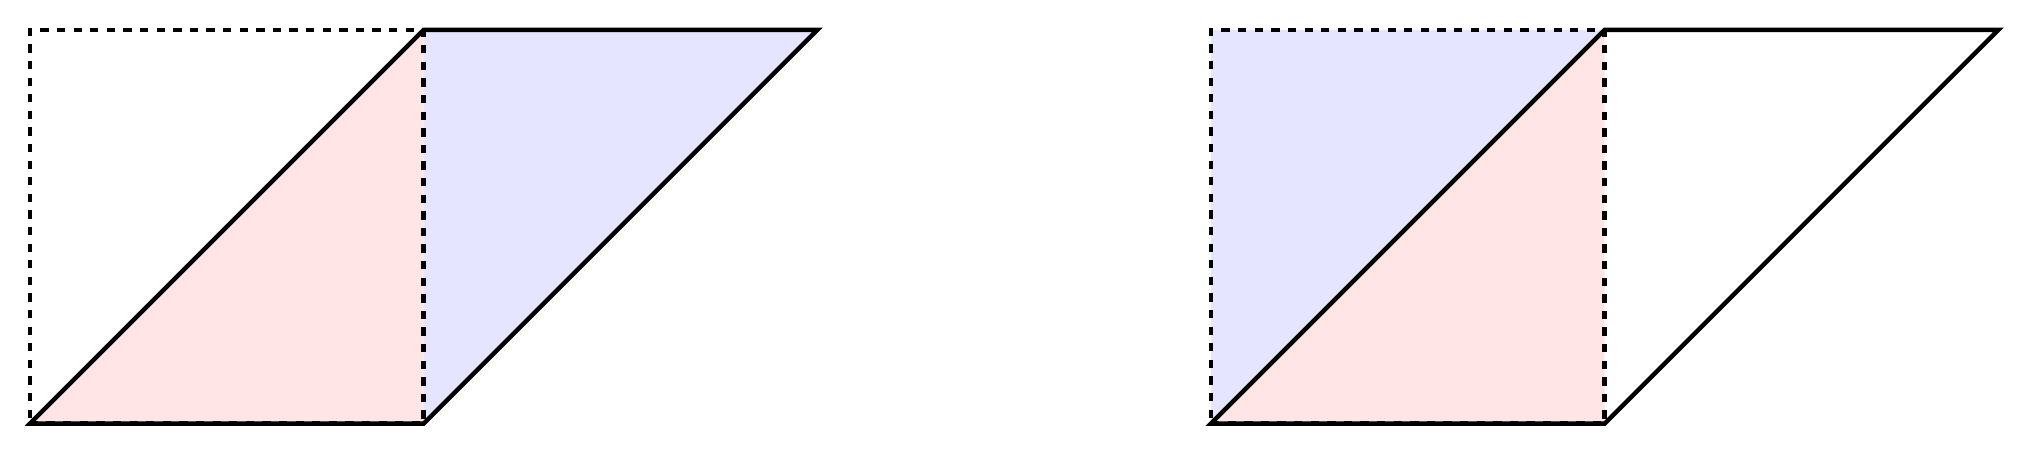
\begin{tikzpicture}

\path[fill=red!10!white] (0,0)--(5,0)--(5,5)--cycle;

\path[fill=blue!10!white] (5,0)--(10,5)--(5,5)--cycle;

%\path[fill=blue!10!white] (0,0)--(5,5)--(0,5)--cycle;

\draw[ultra thick, dashed] (0,0)--(5,0)--(5,5)--(0,5)--cycle;
\draw[ultra thick] (0,0)--(5,0)--(10,5)--(5,5)--cycle;

\begin{scope}[xshift=15cm]

\path[fill=red!10!white] (0,0)--(5,0)--(5,5)--cycle;

%\path[fill=blue!10!white] (5,0)--(10,5)--(5,5)--cycle;

\path[fill=blue!10!white] (0,0)--(5,5)--(0,5)--cycle;

\draw[ultra thick, dashed] (0,0)--(5,0)--(5,5)--(0,5)--cycle;
\draw[ultra thick] (0,0)--(5,0)--(10,5)--(5,5)--cycle;

\end{scope}
\end{tikzpicture}

This in turn has to do with Euclid's Elements.  The shear preserves area, these two rectangles have equal area.  Just take a pair of scissors and cut.

\newpage

\noindent Our goal is to try to express some of these ``entropy" considerations in simple language.  And I need to re-write all of these statements since I am not an expert on Ratner Theorem.


\fontfamily{qag}\selectfont \fontsize{12}{10}\selectfont

\begin{thebibliography}{}

\item Davide Gaiotto, Peter Koroteev \textbf{On Three Dimensional Quiver Gauge Theories and Integrability} \texttt{arXiv:1304.0779}

\item Titchmarsh \textbf{Theory of Functions} \texttt{https://archive.org/details/TheTheoryOfFunctions}



\end{thebibliography}


\end{document}

